%!TEX program = pdflatex
% Full chain: pdflatex -> bibtex -> pdflatex -> pdflatex
\documentclass[11pt,en,bibstyle=unsrt]{elegantpaper}

\title{ElegantPaper: An Elegant \LaTeX{} Template for Working Papers}
\author{Ethan DENG \\ Fudan University \and Dongsheng DENG \\ PA Technology}
\institute{\href{https://github.com/ElegantLaTeX}{Elegant\LaTeX{} Program}}

\version{0.08}
\date{\today}


\begin{document}

\maketitle

\begin{abstract}
This documentation illustrates the usage of the \href{https://github.com/ElegantLaTeX/ElegantPaper}{ElegantPaper} template. This template is based on the standard \LaTeX{} article class, which is designed for working paper writing. With this template, you can get rid of all the worries about the format and merely focus on writing. For any question, please leave a message on \href{https://github.com/ElegantLaTeX/ElegantPaper/issues}{Github::ElegantPaper/issues}. Want to know more about Elegant\LaTeX{} Templates? Please visit: \href{https://github.com/ElegantLaTeX}{https://github.com/ElegantLaTeX}.\par
\keywords{Elegant\LaTeX{}, Working Paper, Template}
\end{abstract}


\section{Introduction}

This template is based on the standard \LaTeX{} article class, hence the arguments of article class are acceptable (\lstinline{a4paper}, \lstinline{10pt} and etc.). Alternative engines are \hologo{pdfLaTeX} and \hologo{XeLaTeX}.

\begin{lstlisting}
\documentclass[a4paper,11pt]{elegantpaper}
\end{lstlisting}
\textbf{Note:} ElegantPaper is available on  \href{https://www.overleaf.com/latex/templates/elegantpaper-template/yzghrqjhmmmr}{Overleaf} and \href{https://gitee.com/ElegantLaTeX/ElegantPaper}{gitee}.

\subsection{Global Options}
Language mode option \lstinline{lang} allows two alternative inputs, \lstinline{lang=en} (default)  for English or \lstinline{lang=cn} for Chinese. \lstinline{lang=cn} will make the caption of figure/table, abstract name, refname etc. Chinese. You can use this option as
\begin{lstlisting}
\documentclass[lang=cn]{elegantpaper} % or
\documentclass{cn}{elegantpaper} 
\end{lstlisting}
\textbf{Note:} Under the English mode \lstinline{lang=en}, Chinese characters are not allowed. To type in Chinese, please load  \lstinline{ctex} or \lstinline{xeCJK} package at the preamble as:
\begin{lstlisting}
\usepackage[UTF8,scheme=plain]{ctex}
\end{lstlisting}

\subsection{Fonts}
This template sets \lstinline{newtxtext} and \lstinline{newtxmath} for English and math fonts respectively.
\begin{equation}
(a+3b)^{n} = \sum_{k=0}^{n} C_{n}^{k} a^{n-k} (3b)^k\label{eq:binom}
\end{equation}

\subsection{Custom Commands}
Default \LaTeX{} commands and environments are all the same in this template\footnote{To ensure the codes are replicatable. We recommend users pay more attention to the contents other than formats. This is the meaning of the existence of the template.}. We created four new commands:
\begin{enumerate}
	\item \lstinline{\email}: create the hyperlink to email address.
	\item \lstinline{\figref}: same usage as \lstinline{\ref}, but start with label text <\textbf{Figure n}>.
	\item \lstinline{\tabref}: same usage as \lstinline{\ref}, but start with label text <\textbf{Table n}>.
	\item \lstinline{\keywords}: create the keywords in the abstract section.
\end{enumerate}


\subsection{Bibliography}
This template used \hologo{BibTeX} to generate the bibliography, the default bibliography style is  \lstinline{aer} under the option \lstinline{lang=en}. Citation example: ~\citep{en1,en2,en3} used data from a major peer-to-peer lending marketplace in China to study whether female and male investors evaluate loan performance differently. 

If you want to use \hologo{BibTeX}, you must create a file named \lstinline{wpref.bib}, and add bib items (from Google Scholar, Mendeley, EndNote, and etc.) to \lstinline{wpref.bib} file, and cite the bibkey in the \lstinline{tex} file. Note that \hologo{BibTeX} has to be added.

Three options for the references, \lstinline{cite=numbers} (default), \lstinline{cite=super} and \lstinline{cite=authoryear}. Those who major in science and engineering use \lstinline{numbers} and \lstinline{super} more often, while those who major in arts use \lstinline{authoryear} more frequently. To switch different options, use
\begin{lstlisting}
\documentclass[cite=super]{elegantpaper} % super style ref style
\documentclass[super]{elegantpaper}

\documentclass[cite=authoryear]{elegantpaper} % author-year ref style
\documentclass[authoryear]{elegantpaper}
\end{lstlisting}

\section{Recruit Support Members}

Recruit support members for Elegant\LaTeX{} to translate template official guide, maintain wiki entries(Markdown), update Wechat articles. No deadline for this recruitment.

So far, Elegant\LaTeX{} has four support members:
\begin{itemize}
	\item OG Translator: \href{https://github.com/peggy2006xzyz}{YPY};
	\item Wiki Maintainer: \href{https://github.com/izinngo}{Ingo Zinngo}, \href{https://github.com/xiaohao890809}{Xiaohao890809};
	\item QQ Group Manager: \href{https://github.com/sikouhjw}{Sikouhjw}.
\end{itemize}

Thank them all!!!

\section{Acknowledgement}
The number of stars on Github for ElegantPaper reached 164 on Oct 17, 2019 at the release of ElegantPaper v0.08.
Thank China\TeX{} and \href{http://www.latexstudio.net/}{\LaTeX{} studio} for their promotion. 

If you like our templates, star on Github.
\begin{figure}[!ht]
	\centering
	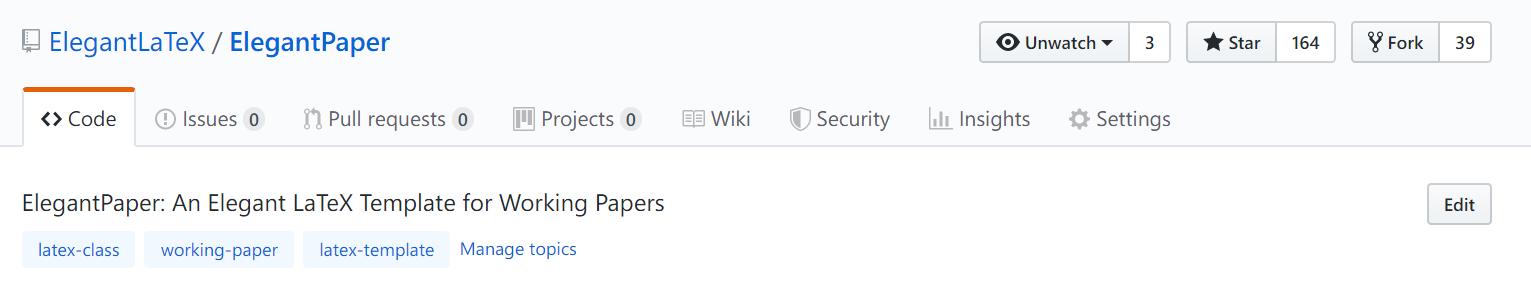
\includegraphics[width=\textwidth]{star.png}
	\caption{Twinkle, Twinkle, Little Star}
\end{figure}

\section{Donation}
To express your love for our templates and/or our developers, please do not hesitate to tip us.
\begin{figure}[!htbp]
	\centering
	
\includegraphics[width=0.4\textwidth]{donate.jpg}
\end{figure}

\textbf{The explanation right of the tip usage belongs to Elegant\LaTeX{} with no supervision. Feel free to tip us.} Those who donate more than 10 RMB will be recorded in the donation list. Thank all the tippers!

\begin{table}[htbp]
	\centering
	\caption{Donation List}
	\begin{tabular}{cccc}
		\toprule
		Tipper   & Amount & Date & Channel \\
		\midrule
		Lerh  & 10 RMB  & 2019/05/15 & Wechat \\
		Yueguodipingxian & 10 RMB   & 2019/05/15 & Wechat \\
		Dapeng & 20 RMB & 2019/05/27 & Wechat\\
		Anonymous & 10 RMB & 2019/05/30 & Wechat \\
		\href{http://www.latexstudio.net/}{latexstudio.net} & 666 RMB & 2019/06/05 & Alipay \\
		Cassis & 11 RMB & 2019/06/30 & Wechat \\
		Some Jun & 10 RMB & 2019/07/23 & Wechat \\
		Some Meng & 19 RMB & 2019/08/28 & Wechat \\
		Qu DouDou & 10 RMB & 2019/08/28 & Wechat \\
		Li Bo & 100 RMB & 2019/10/06 & Wechat\\
		Njustsll & 10 RMB & 2019/10/11 & Wechat \\
		\bottomrule
	\end{tabular}%
\end{table}%

\section{FAQ}

\begin{enumerate}[label=\arabic*).]
	\item \textit{How to remove the information of version?}\\
    Please comment \lstinline|\version{x.xx}|.
	\item \textit{How to remove the information of date?}\\
	Please type in \lstinline|\date{}|.
	\item \textit{How to add several authors?}\\
	Use \lstinline{\and} in \lstinline{\author} and use \lstinline{\\} to start a new line.
	\begin{lstlisting}
	\author{author 1\\ org. 1 \and author 2 \\ org. 2 }
	\end{lstlisting}
	\item \textit{How to display bilingual abstracts?}\\
	Please refer to \href{https://github.com/ElegantLaTeX/ElegantPaper/issues/5}{Github::ElegantPaper/issues/5}
\end{enumerate}

\section{Minimal Example}
A minimal example is as follows:
\begin{lstlisting}
\documentclass[a4paper,11pt]{elegantpaper}

% title information
\title{Working Paper Example}
\author{Author Name} 
\institute{Elegant\LaTeX{} Group}

\version{1.00}
\date{\today}

\begin{document}

\maketitle

\begin{abstract}
Your abstract goes here.
\keywords{keyword1, keyword2}
\end{abstract}

\section{Introduction}
The content of introduction section.

\section{Conclusion}
The content of conclusion section.

\bibliography{wpref}

\end{document}
\end{lstlisting}

\nocite{en1,en2}
\bibliography{wpref}

\end{document}
